\documentclass[aspectratio=169]{beamer}

\usepackage[ngerman]{babel}
\usepackage[utf8]{inputenc}
\usepackage[T1]{fontenc}
\usepackage{tcolorbox}
\usepackage{algpseudocode}
\usepackage{algorithm}
\usepackage{amsmath}
\usepackage{amsfonts}
\usepackage{amssymb}
\usepackage{amsthm}
\usepackage{graphicx}
\usepackage{multicol}
\usepackage{caption}
\PassOptionsToPackage{hyphens}{url}\usepackage{hyperref}
\usepackage{enumerate}
\usepackage{xcolor}
\usepackage{chronology}
\usepackage{tcolorbox}
\usepackage{listings}

\definecolor{mygreen}{RGB}{165, 215, 210}   % UBC Blue (primary)

\usecolortheme[named=mygreen]{structure}
\setbeamercolor{section in sidebar shaded}{fg=black}
\usetheme{Hannover}
\title{sleepCube}
\author{Ugur Turhal, Silvan Lenzlinger \& Berkan Kurt}
\institute{Universit\"at Basel}
\date{\today}

\begin{document}



\frame{\maketitle}
%\frame{\tableofcontents}


\section{Projekt Idee}
\begin{frame}[fragile]
\textbf{Projekt Idee}
\begin{enumerate}[(1)]
\item Etwas was im alltag gebraucht werden kann
\item LED Cube
\item Schlaf-Raumtemperatur
\item CS Studenten \& Schlafmangel
\end{enumerate}
\begin{figure}[!h]
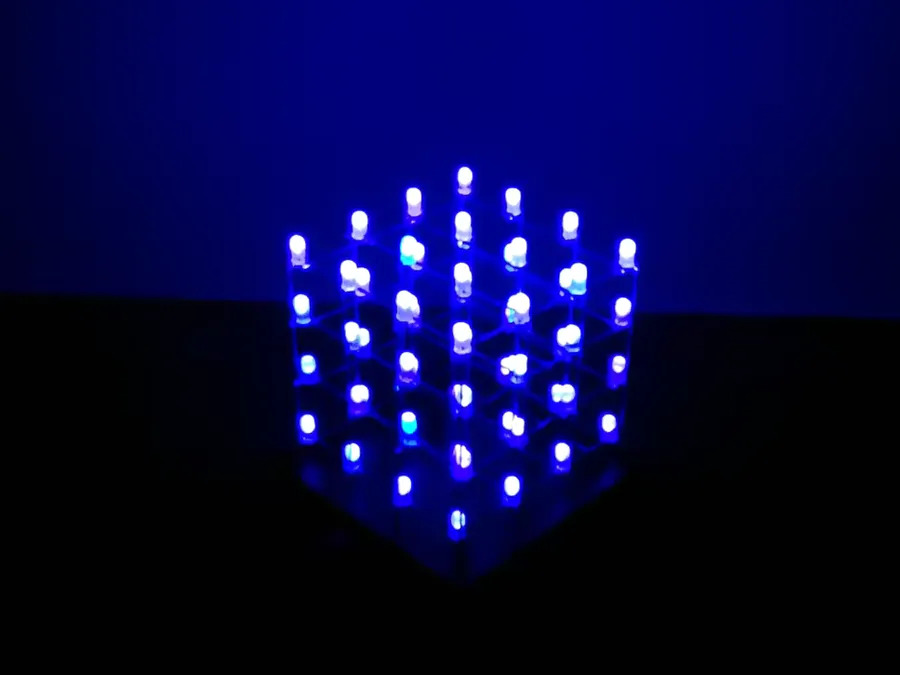
\includegraphics[width=0.4\textwidth]{cube.jpg}
\captionof{figure}{4 $x$ 4 $x$ 4 - LED Cube\footnote{\url{https://www.hackster.io/ProMaker_101/4x4x4-led-cube-making-d71684}}} \label{cube} 
\end{figure}
\end{frame}



\section{sleepCube - INFOS} 
\begin{frame}[fragile]
\textbf{sleepCube - INFOS}
\begin{columns}
\begin{column}{0.5\textwidth}
\begin{itemize}
\item Mikrocontroller: Arduino UNO ATMega328
\item Cube Grösse:  4 $\times$ 4 $\times$ 4
\item LED Farben: \textcolor{red}{Rot} \& \textcolor{green}{Grün}, \underline{keine} RGB LEDs

\end{itemize}

\end{column}

\begin{column}{0.5\textwidth}
\begin{itemize}
\item DHT22 für Temperaturmessgerät
\item Genauer als TMP36
\item \textcolor{red}{Rot-Leuchten} $<$15$^{\circ}$ C oder $>$18$^{\circ}$ C
\item \textcolor{green}{Grün-Leuchten} $\geq$15$^{\circ}$ C oder $\leq$18$^{\circ}$ C
\end{itemize}
\end{column}

\end{columns}
\end{frame}

\section{Mögliche Schwierigkeiten} 
\begin{frame}[fragile]
\textbf{Mögliche Schwierigkeiten}
\begin{itemize}
\item Sauberes Löten
\item Symmetrischer Cube z.B. Abstände
\item Ästhetik
\item Gestell (Gehäuse z.B. aus Plexiglas)
\item Digitaler Temperatur Sensor (Noch nie benutzt)
\end{itemize}
\begin{columns}
\begin{column}{0.45\textwidth}


\end{column}
\begin{column}{0.5\textwidth}

\end{column}

\end{columns}
\end{frame}


\section{Timeline} 
\begin{frame}[fragile]
\textbf{Timeline}
\begin{figure}

\begin{tikzpicture}[scale=0.5,every node/.style={outer sep=5pt}]
    %Notation: {year, the title of the event}
    %NOTE! Everyting is zero-based
    \def\ourInfo{{
        {"5. Dezember","Ugur: DHT und LEDs Testen auf Breadboard"},
        {"10. Dezember","Silvan \& Berkan überlegen Aufbau"},
        {"20. Dezember","Aufbau umsetzen: Löten etc."},
        {"24. Januar 2022","Abgabe"},
    }}
    \pgfmathsetmacro{\length}{3}% Zero based.

    % Loop through the array containing all events.
    \foreach \i in {0, ..., \length}{
        \pgfmathsetmacro{\year}{\ourInfo[\i][0]}% Get the left cell (year)
        \pgfmathsetmacro{\eventName}{\ourInfo[\i][1]}% Get the right cell (event name)
        \draw[thick,mygreen] (0,-2*\i-2)--(0,-2*\i);% Draw vertical line
        \ifnum \i=1 % Should be in red text
          \draw(0,-2*\i-1) node[black, right, align = left]{\eventName};% Display the event name
          \draw(0,-2*\i-1) node[black, left] {\year};
        \else % Should be in black text
           \draw(0,-2*\i-1) node[right, black]{\eventName};% Display the event name
           \draw(0,-2*\i-1) node[left] {\year};% Display the year
        \fi
    }
    % Draw the bullet with the dash
    \foreach \i in {0, ..., \length}{
        \filldraw[draw = white, fill = mygreen,thick] (0,-2*\i-1) circle (5pt);
        \draw[thick,mygreen] (-12pt,-2*\i-1)--(0,-2*\i-1);
    }
\end{tikzpicture}
\end{figure}
\end{frame}

\section{Fragen} 
\begin{frame}[fragile]
\textbf{Fragen}

\begin{center}
Fragen?
\end{center}

\end{frame}

\end{document}